\documentclass[
reprint,
%superscriptaddress,
%groupedaddress,
%unsortedaddress,
%runinaddress,
%frontmatterverbose,
%preprint,
preprintnumbers,
%nofootinbib,
%nobibnotes,
%bibnotes,
 amsmath,
 amssymb,
 aps,
onecolumn,
prd,
%prb,
%rmp,
%prstab,
%prstper,
%floatfix,
]{revtex4-2}

\usepackage{graphicx}% Include figure files
\usepackage{dcolumn}% Align table columns on decimal point
\usepackage{bm}% bold math
%\usepackage{hyperref}% add hypertext capabilities
%\usepackage[mathlines]{lineno}% Enable numbering of text and display math
%\linenumbers\relax % Commence numbering lines
%\usepackage[showframe,%Uncomment any one of the following lines to test
%%scale=0.7, marginratio={1:1, 2:3}, ignoreall,% default settings
%%text={7in,10in},centering,
%%margin=1.5in,
%%total={6.5in,8.75in}, top=1.2in, left=0.9in, includefoot,
%%height=10in,a5paper,hmargin={3cm,0.8in},
%]{geometry}
\usepackage{xcolor}
\usepackage{textcomp,gensymb}
\begin{document}

%\preprint{APS/123-QED}

\title{Neutrino Oscillation and its impact on the r-process in Neutron Star merger remnants}% Force line breaks with \\
%\thanks{A footnote to the article title}%

%\author{Xilu~Wang}
%\author{Y. L.~Zhu}
%\email{yzhu14@ncsu.edu}
%\author{G. C.~McLaughlin}
%\author{Rebecca Surman}
%\email{Gail_McLaughlin@ncsu.edu}
%\author{Albino Perego?}

\date{\today}% It is always \today, today,
             %  but any date may be explicitly specified

\begin{abstract}

\end{abstract}

%\keywords{Suggested keywords}%Use showkeys class option if keyword
                              %display desired
\maketitle
\section{Type of neutrino oscillation}
\begin{equation}
i \frac{d}{d t} S(\Omega, q, \mathbf{x}, t)=\left(H_{V}(q)+H_{e}(\mathbf{x}, t)+H_{\nu \nu}(\mathbf{x}, t)\right) S(\Omega, q, \mathbf{x}, t)
\end{equation}
\subsection{Vacuum}
\subsection{MSW}
\subsection{Bipolar}
\subsection{Matter-Neutrino Resonance}
\begin{figure}[!h]
  \centering
  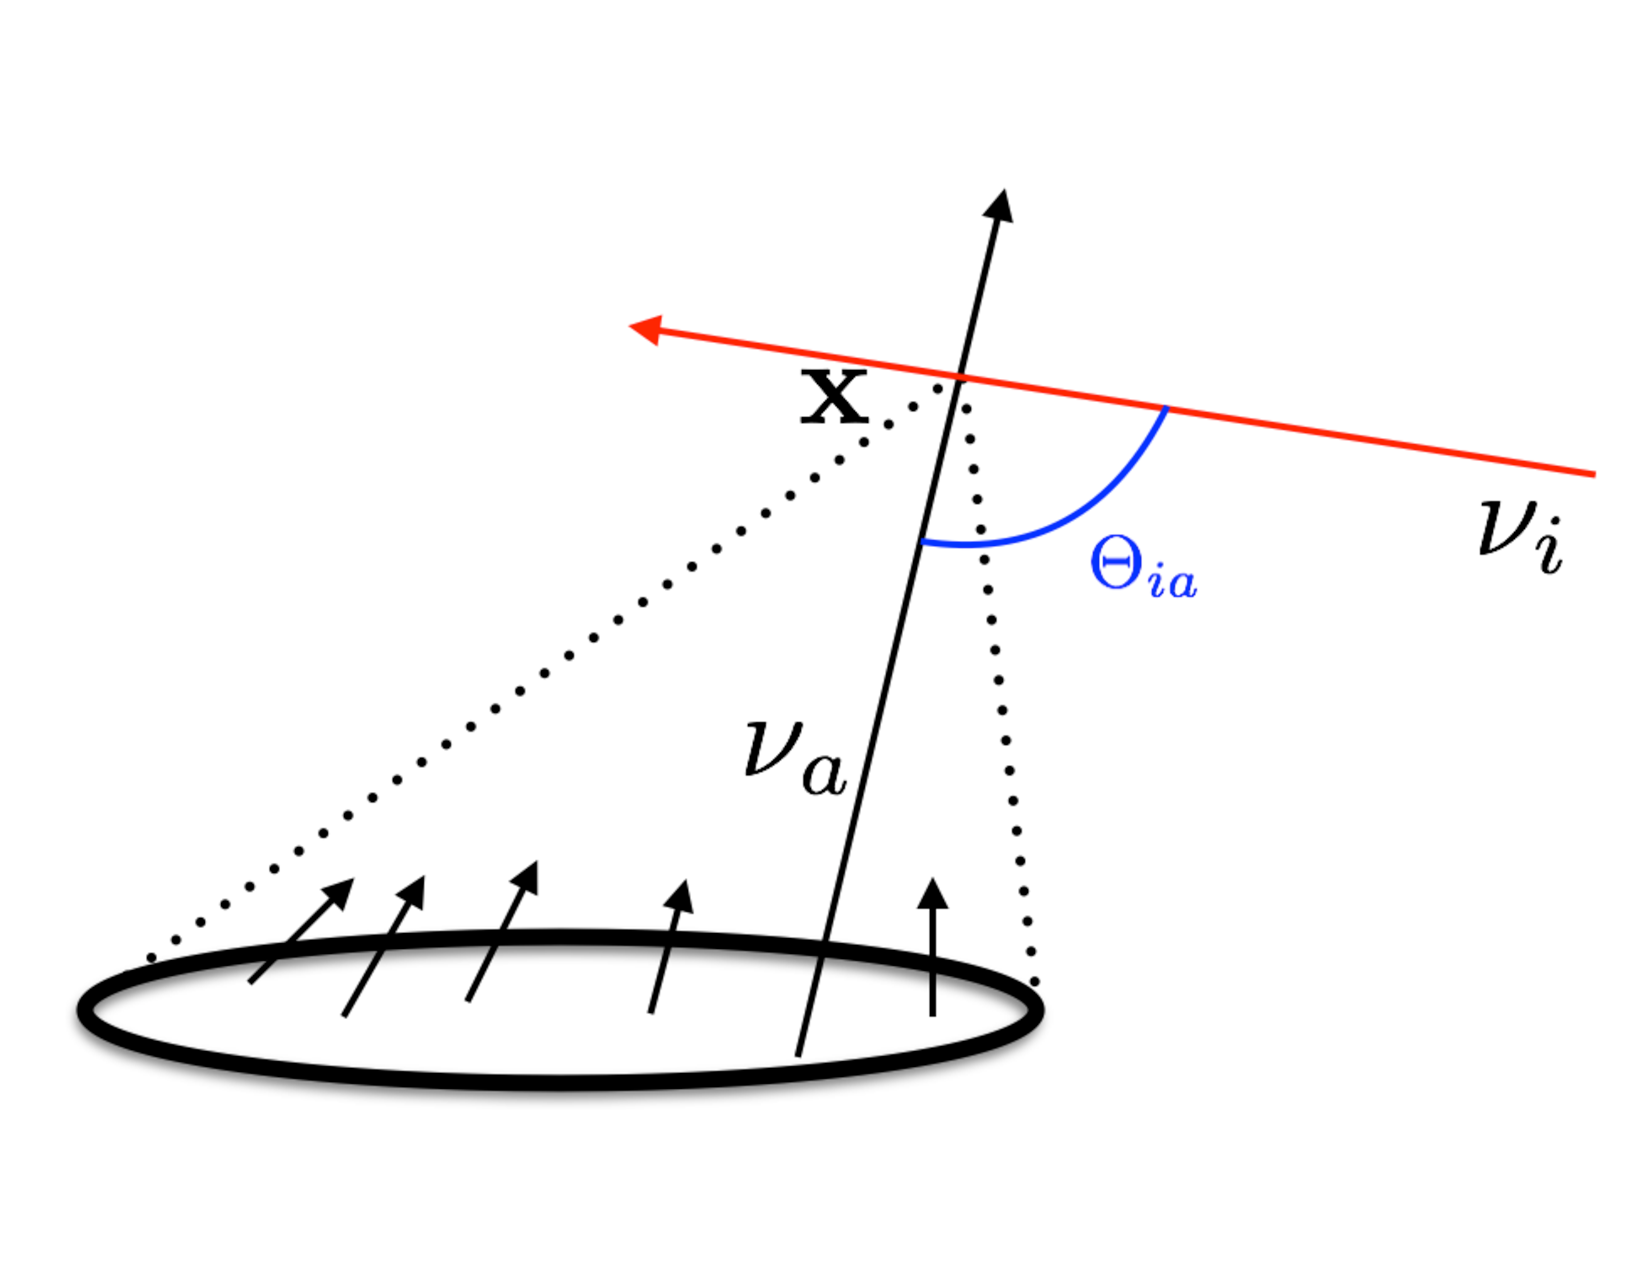
\includegraphics[width=0.6\textwidth]{neutrinointeraction.pdf}
  \caption{\label{fig:neutrinointeraction}
  (Cite phd thesis)
  Scheme of neutrino self-interaction above compact object mergers.
  The neutrino $\nu_\alpha$ represents the environmental neutrino or antineutrino emitting out of the accretion disk. 
  The red arrow represents the propagating trajectory of neutrino $\nu_i$ and the black arrows represent the trajectories of neutrino and antineutrinos.
  The neutrino $\nu_i$ represents the observing neutrino, which intersects with $\nu_\alpha$ of angle $\Theta_{ia}$. 
  }
\end{figure}
The hamiltonian that describes neutrino self-interaction $H_{\nu\nu}$, can be included the Hamiltonian $H$,
\begin{equation}
H_{\nu\nu} =\sqrt{2}G_F \int_0^{+\infty} dq \int_\Omega (1- cos{\Theta_{ia}}) (\rho_\nu d n_\nu - \rho_{\bar{\nu}} d n_{\bar{\nu}}),
\end{equation} 
where $\rho_\nu$($\bar{\rho}_\nu$) denotes the neutrino(anti-neutrino) density matrix and $d n_\nu$($d n_{\bar{\nu}}$) is the infinitesimal of the local neutrino(anti-neutrino) density.
\begin{equation}
\begin{aligned} 
H_{\nu \nu}(\mathbf{x}, t)
=& \sqrt{2} G_{F} \int_{0}^{\infty} d q \int_{\Omega}\left(1-\cos \Theta_{ia}\right) \left(\rho_{\nu}(\Omega, q, \mathbf{x}, t) d n_{\nu}(\Omega, q, \mathbf{x}, t)\right. \left.-\rho_{\bar{\nu}}(\Omega, q, \mathbf{x}, t) d n_{\bar{\nu}}(\Omega, q, \mathbf{x}, t)\right) 
\end{aligned}
\end{equation}
\begin{equation}
\begin{array}{l}
\rho_{\nu}(\Omega, q, \mathbf{x}, t)= S(\Omega, q, \mathbf{x}, t) \rho_{\nu}(\Omega, q, \mathbf{x}, 0) S^{\dagger}(\Omega, q, \mathbf{x}, t) . 
\end{array}
\end{equation}

\begin{equation}
\begin{aligned} 
\frac{H_{\nu \nu}(\mathbf{x}, t)}{\sqrt{2} G_{F}}=& \int_{0}^{\infty} d q \int_{\Omega}\left(1-\cos \Theta_{ia}\right)\left(\rho_{\nu}(\Omega, q, \mathbf{x}, t) d n_{\nu}\right.\left.(\Omega, q, \mathbf{x}, t)-\rho_{\bar{\nu}}(\Omega, q, \mathbf{x}, t) d n_{\bar{\nu}}(\Omega, q, \mathbf{x}, t)\right) 
\end{aligned}
\end{equation}
\begin{equation}
d n_{\nu(\bar{\nu})}(\Omega, q, \mathbf{x}, t)=\frac{\Phi_{\nu(\bar{\nu})}(q) d \phi d(\cos \theta)}{4 \pi}
\end{equation}
\begin{equation}
\begin{aligned} 
\\\frac{4 \pi H_{\nu \nu}(\mathbf{x}, t)}{\sqrt{2} G_{F}}=& \int_{0}^{\infty} d q\int_{\Omega} \left( \Phi_{\nu}(q) \left(1-\cos \Theta_{ia}\right) \rho_{\nu}(\Omega, q, \mathbf{x}, t)  -\Phi_{\bar{\nu}}(q) \left(1-\cos \Theta_{ia}\right)  \rho_{\bar{\nu}}(\Omega, q, \mathbf{x}, t) \right)  d \phi d(\cos \theta) 
\end{aligned}
\end{equation}
\subsection{Instability}

\section{Method}
\subsection{Tracers from hydro}
Albino shared the tracer particle trajectory files as in~\citet{Martin2015NEUTRI}.
They distinguished between four different angular bins and three "ejection times".
For each combination, Albino sent a "representative tracer", which is close to the average behavior in Fig.~7 in ~\citet{Martin2015NEUTRI}.
\begin{table}[b]
    \caption{\label{tab:table1}}
    \begin{ruledtabular}
        \begin{tabular}{ccccc}
            \textrm{Timescale(ms)\footnote{Timescale after merge.}}&
            \textrm{Bin 1: $0\degree - 15\degree$}&
            \textrm{Bin 2: $15\degree - 30\degree$} &
            \textrm{Bin 3: $30\degree -45\degree$} &
            \textrm{Bin 4: $45\degree- 60\degree$}\\
            \colrule
            90 & 01407 & 57221 & 16463 & 32228 \\
            140 & 78323 & 69686 & 37655 & 26091 \\
            190 & 66394 & 61778 & 79049 & 80224 \\
        \end{tabular}
    \end{ruledtabular}
\end{table}

The tracer numbers are associated to the following bins and times in Table.~\ref{tab:table1}.
Each tracer is a Lagrangian particle that records the local values of the most relevant quantities (radius, density, temperature,...) as a function of time along the particle trajectory $\mathbf{x}=\mathbf{x}(t).$
The values reported are the ones provided by Albino's 3D simulations.

\textbf{TODO: Check how the position vectors are obtained.}

%The first patch of files contains only the radius as a function of time, but I think in the future we will need the full position vector, since the oscillation patter has a strong geometrical dependence.
We have the corresponding final nuclear abundances, which is obtained by Dirk using the Winnet network.
This network has also some neutrino reactions implemented, which require some neutrino quantities from the simulation (luminosity and mean energy).

\textbf{TODO: Check with Albino about how the \it{neutrino reactions implemented.}} 

Albino said that he expects the differences to be marginal (both in Ye and in the final nuclear abundances), because the change in Ye is usually small after NSE freeze-out.
To get an idea, you can compare the Ye at NSE freeze out with the final one (since the network reproduces quite well the Ye from the simulation after NSE freeze-out).

\textbf{TODO: Check how Dirk handled the NSE.} 

\textbf{TODO: no SDF in Dirk's calculation?}
\subsection{Preparation of Tracers}
Extropolate Tracers.

NSE/temperature
\subsection{Neutrino Treatment}

\subsubsection{Neutrino Captrue Rate}
To include the neutrino oscillation impact in the nucleosynthesis calculation, we use the oscillated neutrino density to calculate the rate per solid angle for electron neutrino captures on free neutrons with both the oscillated and unoscillated neutrino spectra as in Ref.~\cite{Frensel2017Neutri}
The oscillated rate is given by:
\begin{equation}
R_{\nu_e,n}(r) = \frac{1}{4\pi} \sum_{\alpha=e,\mu,\tau} F_{\nu_\alpha} \int_0^\infty dE f_{\nu_\alpha}(E) \delta_{\nu_e,n,abs}(E) P(\nu_\alpha \to \nu_e)(E,r).
\end{equation}

\subsection{Pseudo-multi angle}
We pick trajectories in $nA$ angular bins for any point on the tracer, and perform multi-energy/single angle calculation for each trajectories and used the updated neutrino flux from each energy and each angular bin to calculated the neutrino capture rate.
\\
Remark: 
\begin{itemize}
\item This method may be very computational expense to get a oscillated neutrino density profile in the NS merger remnants. But for the reaction network nucleosynthesis calculation, we just need neutrino capture rate along the tracers.
\item This method is not very bad because in the NS merger remnant simulation we use, the matter density in very high for the early part of all neutrino trajectory. The matter suppress almost all oscillation before they encounter the condition for MNR(Need to be validated). If that is true, the only part we need to worry is the multiangle effect the endpoint of MNR, for reaction network calculations. We may need to figure out a way to verify that(bulb model?, See Alexey's paper?).
\end{itemize}

\subsubsection{Ray-tracing neutrinos along the tracers}
Point sampling on the tracer.

Neutrino trajectory ray-tracing.







\begin{acknowledgments}
\dots.

\end{acknowledgments}

\appendix

\section{Recent Advancement}
\citet{Li2021Neutri} treat fast flavor conversion as in \citet{Sarikas2012Suppre}.

\section{Neutrino Oscillation with Simulated Neutrino Density}
\subsection{\label{sec20u}Preparation}
The simulation of the aftermath of a binary neutron star merger, under the influence of neutrino heating and cooling, gives the matter properties and the specific neutrino densities in a certain point in space, for a specific neutrino flavor and energy bin.
The specific neutrino densities $F_{\mathbf{x}, \nu, E}(\theta, \phi)$ on a plane characterized by an constant azimuthal angle $\phi_0$. So the local neutrino density $n_\nu(\mathbf{x})$ ($particles/cm^3$) can be calculated as
\begin{equation}
n_\nu(\mathbf{x})=
\int_0^{+\infty}\left(\int_\Omega F_{\mathbf{x}, \nu, E}(\theta, \phi)\,d\Omega \right)\,E^2\,dE.
\label{eq:localDensityOfSpecificNeutinoDensities}
\end{equation}
Thus, $F_{\mathbf{x}, \nu, E}(\theta, \phi)$has the units of $particles/cm^3/stead/MeV^3$. The local density can also be calculated from the neutrino distribution function, $f_\nu$, as
\begin{equation}
n_\nu(\mathbf{x})=\frac{1}{\left(2\pi\hbar\right)^3}\int_{R^3} f_\nu(\mathbf{x}, \mathbf{p})\,d^3\mathbf{p}.\label{eq:localDensitiesOfDistribution}
\end{equation}
In spherical coordinates,$d^3\mathbf{p}=p^2\,dp\,d\Omega$, and $E=pc$, we can write
\begin{equation}
n_\nu{\left(\mathbf{x}\right)}=\frac{1}{(2\pi\hbar c)^3}\int_0^{+\infty}\left(\int_\Omega f_\nu(\mathbf{x},E,\theta,\phi)\,d\Omega\right)E^2\,dE.
\end{equation}
Then, then quantity from the output, specific neutrino densities $F_{\mathbf{x},\nu,E}(\theta,\phi)$, expressed in terms of the neutrino distribution functions, corresponds to 
\begin{equation}
F_{\mathbf{x},\nu,E}(\theta,\phi) \equiv \frac{f_\nu(\mathbf{x},E,\theta,\phi)}{(2\pi\hbar c)^3}.
\end{equation}
The neutrino type is distinguished as $\nu_e,\bar{\nu}_e$, and $\nu_{\mu,\tau}$. The neutrino energy has been discretized in 8 logarithmically increasing energy bins, ranging from $2$ MeV up to $37.45$ MeV ($12$ bins to $200$ MeV in the hydro simulations). The solid angle has been divided into $N_\theta \times N_\phi$ portions. Along $\phi$, $N_\phi=12$ is chosen and equally spaced between $0$ and $2\pi$. Along $\theta$, $N_\theta=6$ is chosen and angeles between	 $0$ and $\pi$ equally spaced with respect to $\cos \theta$. So our angular resolution is $\delta \phi \times \delta \cos \theta =\delta \Omega =4\pi/(N_\theta\times N_\phi)$. In a few words, $F_{\mathbf{x},\nu,E}(\theta,\phi)\,E^2 \,\delta E\,\delta\Omega$ is the amount of neutrinos of flavor $\nu$, with energy in an interval $E\,\pm\,\delta E/2$, that at the point $\mathbf{x}$ moves inside a cone of amplitude $\delta\Omega$, of vertex in $\mathbf{x}$ and axis along $(\theta, \phi)$. The angles $\theta$ and $\phi$ are measured with respect to a local reference frame $\mathbf{O}_{\mathbf{x}}xyz$. But all these local reference frames are parallel among them. And the $z$ axis are parallel to the rotational axis of the HMNS and of the disc.
%########
First, we try to replicate the work in Ref.~\citet{Martin2016Impact} with {\it Prism} code.
Yonglin got tracers from Albino in Ref.~\citet{Martin2016Impact} with Cartesian coordinates. 
\\
In nu.potentials.v2, the two ouput files are density and potential. The density files are defined as
\begin{equation}
dn(\mathbf{x},E	) = E^2\,dE \int_\Omega F_{\mathbf{x}, \nu, E}(\theta, \phi)\,d\Omega.
\end{equation}
with units $particles/cm^3$. The potential files are 
\begin{equation}
dl(\mathbf{x},E	) = E^2\,dE \int_\Omega \left(1-\cos \Theta \right)F_{\mathbf{x}, \nu, E}(\theta, \phi)\,d\Omega.
\end{equation}
Then, with Yonglin's script inputNu.py, we get
\begin{equation}
\delta n(x_i,E_i)=E_i^2\,\delta E_i \int_\Omega F_{\mathbf{x}, \nu, E_i}(\theta, \phi)\,d\Omega.
\end{equation}
\begin{equation}
\delta p(x_i,E_i)=\sqrt[]{2} G_F E_i^2\,\delta E_i \int_\Omega \left(1-\cos \Theta \right)F_{\mathbf{x}, \nu, E_i}(\theta, \phi)\,d\Omega.
\end{equation}
with give,
\begin{equation}
N(x)=\sum \delta n(x_i,E_i)\,
\end{equation}
\begin{equation}
P(x)=\sqrt[]{2} G_F \sum \delta l(x_i,E_i)
\end{equation}

\subsection{Nuclear Statistics equilibrium}
We use a constant entropy calculated from the last line of the tracers. Use the free expansion to calculate the density first. Use the constant Ye of the last line of tracer. Use their dynamicYe.h to calculate Temperature.
Here is the question,
How to get constant entropy? How to get the Temperature.

In Ref.~\citet{Meyer1994Ther}, the entropy of a given thermally isolated system with constant volume is,
\begin{equation}
S = k \,ln\, \Gamma 
\end{equation}
where the $k$ is the Boltzman constant and $\Gamma$ is the number of energetically allowed macroscopic states available to the system.
The system will reach the equilibrum at its maximum entropy and experience no further evolution.
In this NSE, if we combine free neutrons and protons into nuclei, we decrease the number of free particles of the system. 
This would yield fewer ways of sharing the total energy of the system and thus decrease the number of macroscopic states avaible. 
The nuclear reactions also release binding energy, however, which increases the number of photons in the system, the energy available to the leptons and the excitation energy in the nuclei.
This effects increase the number of ways of the system can share the total energy of the system and, hence, can increase the number of macroscopic states available to the system. 
This increase can more than compensate for the decrease in the number of states due to the loss of free particles and can lead to an increase in the entropy. 
Once the system has evolved to the point that it experiences no net increase in the number of macroscopic states by changing the abundance of any particular nucleus, the system has reached NSE.  
If the system expands adiabatically, the temperature will decrease. 
To reach the equilibrium, binding energy released from nuclear reactions heats up the system and tends to counter the temperature decrease from the expansion, until finding a new equilibrium. 
Therefore, in building up the abundances of heavy nuclei, entropy is transferred from the baryons to the photons and leptons.
After all the binding energy has released, the electron-positron pairs annihilation creates two photons, which transfers entropy from the electron-positron pairs into the photons adiabatically. 
At late times, after the electron-positron pairs annihilated, some residual of electrons in the system is left to keep charge neutrality. 
Now, the system is a mix of relativistic photons \textcolor{red}{isn't there any neutrinos?} and nonrelativistic nuclei and electrons.
For the adiabatic expansion, $\rho \propto T^3$ for relativistic particles and $\rho \propto T^{3/2}$ for nonrelativistic particles. 
With the mixture of this two particles, the system actually expands such that $\rho \propto T^b$ where $b$ is between $3/2$ and $3$. 
\textcolor{red}{In~\citet{Martin2016Impact,Korobkin2012Onthe},they use free expansion for the density and adiabatic expansion for the temperature.}
The nuclei will continue to increase in mass until they have reached the nuclides with the largest binding energy per nucleon.
% * <zhu.yonglin3@gmail.com> 2016-11-07T15:50:30.633Z:
%
% ^.
\bibliography{ref}% Produces the bibliography via BibTeX.

\end{document}
%
